\documentclass{article}
\usepackage[utf8]{inputenc}
\usepackage[legalpaper, portrait, margin=0.5in]{geometry}
\usepackage[spanish,es-tabla]{babel}

\title{Trabajo Práctico 1: Conceptos básicos}
\author{Emanuel Ferreyra, Bruno Kaufman, Ariel Salgado}
\date{\today}

\usepackage{natbib}
\usepackage{graphicx}

\begin{document}

\maketitle


\section{Problema 1}
En este punto se pide analizar tres redes complejas de interacción de proteinas. La primera se trata de interacciones binarias entre proteinas, la segunda de co-pertenencia a complejos, y la tercera una obtenida del proyecto Yeast Interactome Database (YID).

\subsection{Punto 1.a.}
En este inciso se solicita visualizar las redes de forma informativa acerca de su estructura. Las tres redes se visualizan en la tabla \ref{comparacionvisualP1}.
%% Fijate de incluir una mención a cada red en el texto, que no esté solo en la figura. Y también poner las redes "completas", no cortadas en dos.
\begin{table}[ht]
\caption{\textbf{Superior:} Componente gigante perteneciente a la red del proyecto YID (Y2H), de interacciones binarias (APMS), y de co-pertenencia (LIT), de izquierda a derecha. \textbf{Inferior:} misma información respecto a las componentes pequeñas de las redes.}
\centering
\begin{tabular}{ccc}
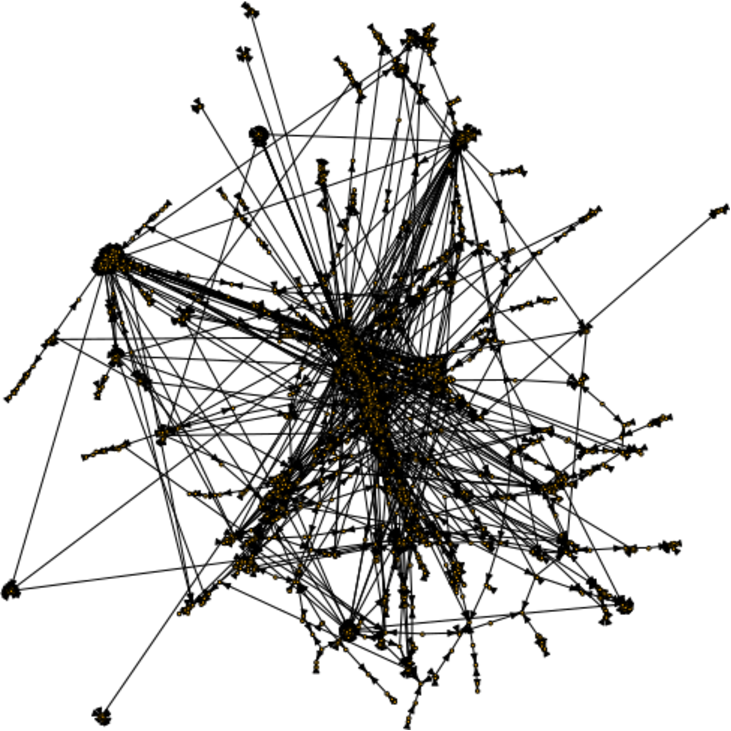
\includegraphics[scale=0.4]{Imagenes_P1/Y2Hgigante.pdf}&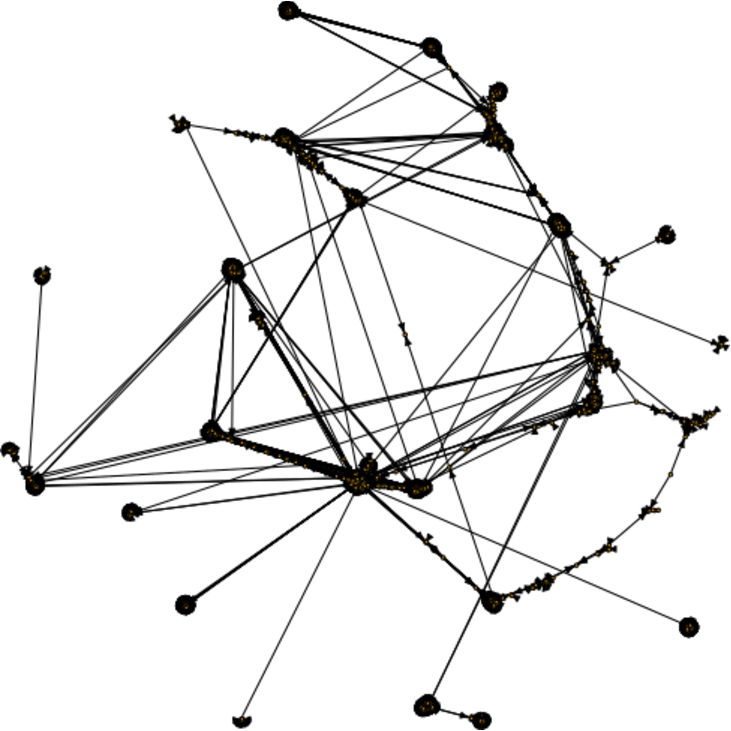
\includegraphics[scale=0.4]{Imagenes_P1/APMSgigante.pdf}&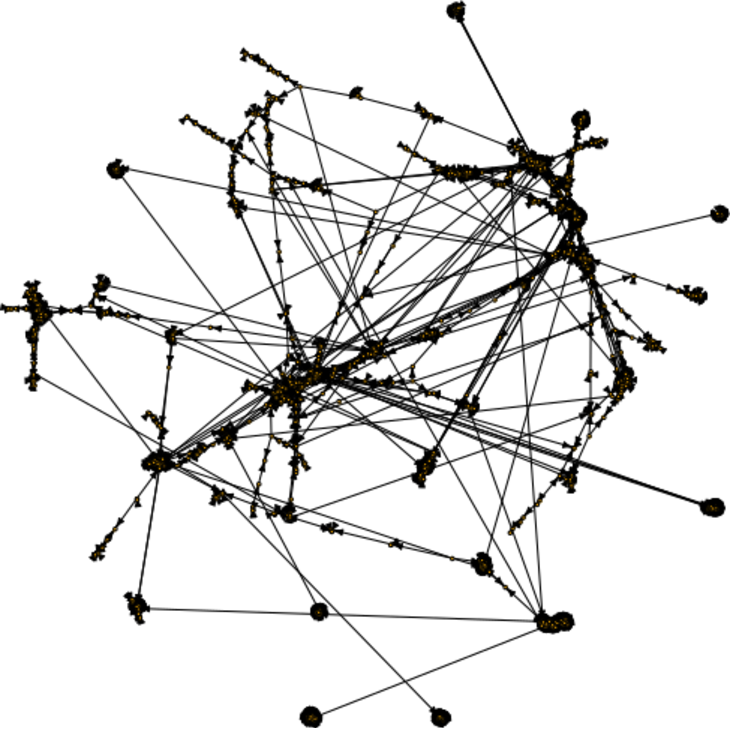
\includegraphics[scale=0.4]{Imagenes_P1/LITgigante.pdf}\\
 
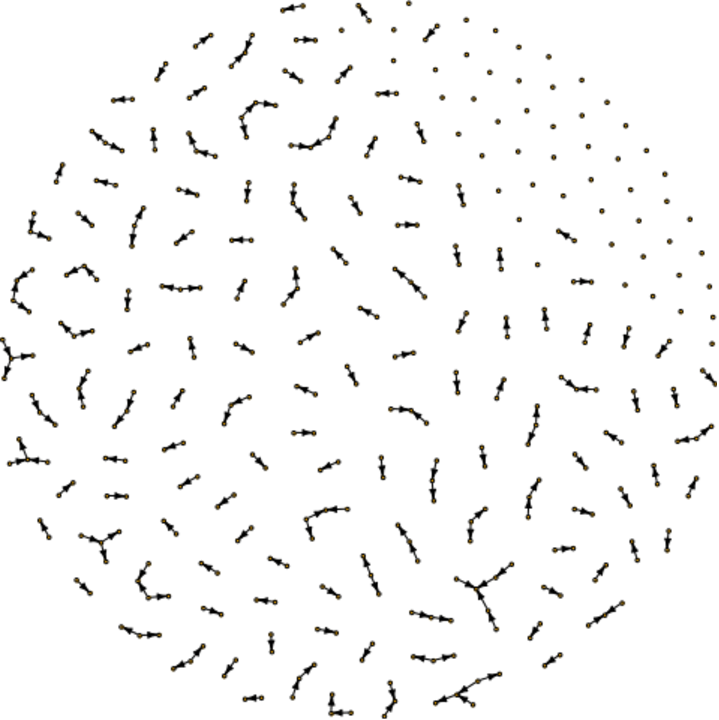
\includegraphics[scale=0.4]{Imagenes_P1/Y2Hchiquitos.pdf}&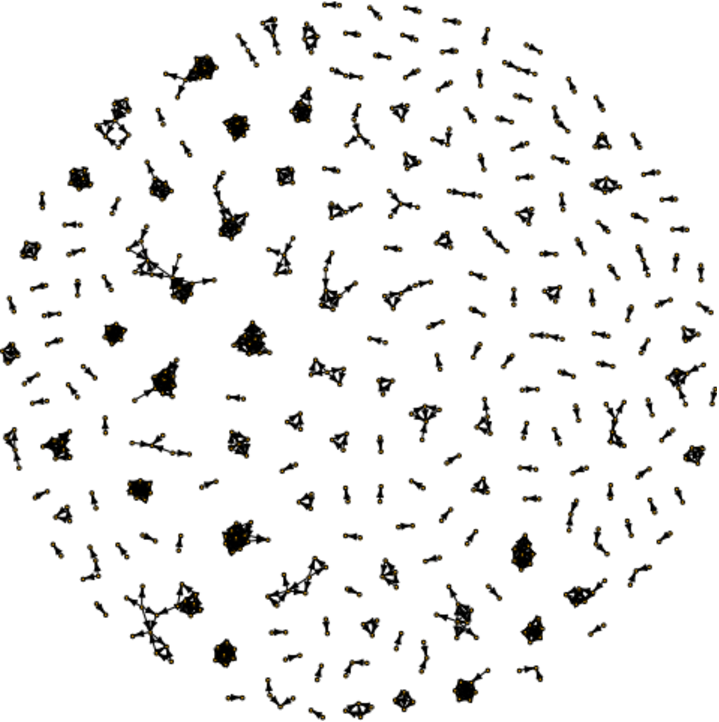
\includegraphics[scale=0.4]{Imagenes_P1/APMSchiquitos.pdf}&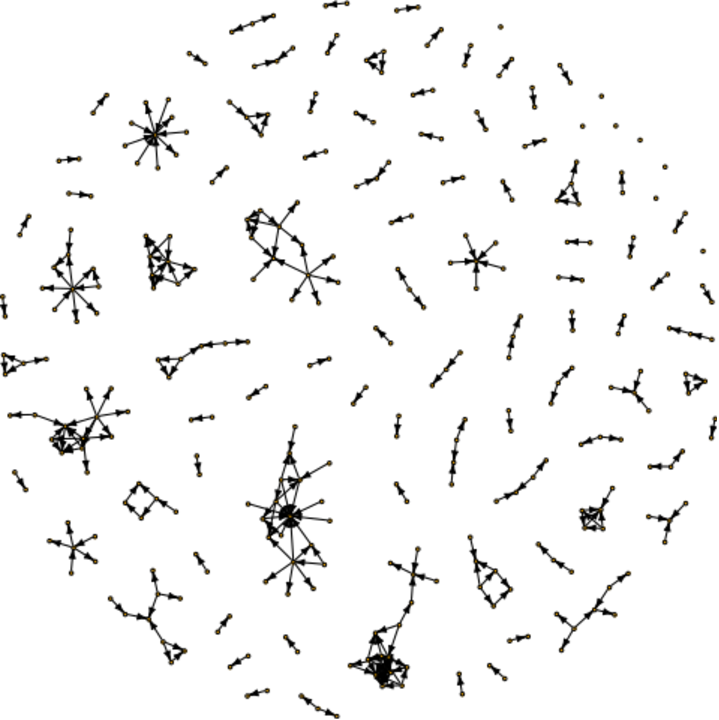
\includegraphics[scale=0.4]{Imagenes_P1/LITchiquitos.pdf}\\
\end{tabular}
\label{comparacionvisualP1}
\end{table}

Se pueden observar algunas cosas en base a estos diagramas. En primer lugar, observando sólamente a los componentes pequeños podemos ver que en la red Y2H, no presentan clustering considerable. En contraste, la red APMS presenta clustering significativo, y la red LIT también, aunque no tanto como la red APMS.

Por otro lado, observando el componente gigante se puede ver que la mayoría de los links de la red Y2H tienden hacia un mismo lugar en la red, mientras que la red APMS se presenta menos centralizada y la LIT toma un punto medio entre las dos.

\subsection{Punto 1.b.}
En este inciso se pide resumir ciertas características de red en una tabla. La siguiente se puede ver en la tabla \ref{tablacantidadesredesP1}.

\begin{table}[ht]
\caption{Cantidades de red asociadas a las redes correspondientes.}
\centering
\resizebox{400pt}{!}{%
\begin{tabular}{lccc}
\textbf{Red} & \textbf{Y2H} & \textbf{APMS} & \textbf{LIT}\\
Número de nodos & 2018 & 1622 & 1536\\
Número de ejes & 2930 & 9070 & 2925\\
Grado medio & 2.904 & 11.184 & 3.809\\
Densidad & 1.440 10\textsuperscript{-3} & 6.899 10\textsuperscript{-3} & 2.481 10\textsuperscript{-3}\\
Clustering global & 2.361 10\textsuperscript{-2} & 6.186 10\textsuperscript{-1} & 3.462 10\textsuperscript{-1}\\
Clustering local medio & 9.700 10\textsuperscript{-2} & 7.410 10\textsuperscript{-1} & 4.556 10\textsuperscript{-1}\\
Diámetro & 14 & 15 & 19\\

\end{tabular}}
\label{tablacantidadesredesP1}
\end{table}

Se puede ver que efectivamente la red Y2H presenta un clustring significativamente menos a las otras dos, y que la APMS tiene uno mayor a la red LIT, aunque están en el mismo órden de magnitud.

Además, es interesante ver que el diámetro nos informa que para llegar de un extremo al otro de la red LIT, el número máximo es apreciablemente mayor que en las otras dos. Esto no es fácilmente visible en los diagramas vistos en la tabla \ref{comparacionvisualP1}

\subsection{Punto 1.c.}

Las interacciones reportadas son todas de naturaleza biomolecular. Por un lado, es razonable que exista una sola componente gigante para estas redes, ya que las redes biológicas presentan una distribución de grado libre de escala, consistente con un mecanismo de attachment preferencial: en otras palabras, cuanto mayor el grado de un nodo, mayor la probabilidad de que tenga un dado enlace con otro. Entonces, la componente más grande siempre atraerá la mayoría de los enlaces, y se volverá más grande, llegando a ser la única componente gigante. Además, se espera en todos los casos la presencia de pocos hubs con grado significativamente mayor a la mayoría, al ser la distribución de grado libre de escala.

Por otro lado, es razonable que una red de co-pertenencia (LIT) tenga una clusterización significativa, ya que muchas proteínas pueden pertenecer a un mismo complejo, y así todas estarán conectadas entre si formando un clique. Suponiendo que esta co-pertenencia influye sobre las interacciones binarias, tiene también sentido que una clusterización alta se presente en la red de interacciones binarias (APMS).

Además, la red de copertenencia (LIT) presenta un diámetro más grande que las otras dos. Esto es razonable, porque cuando se trata de interacciones binarias (APMS, Y2H), es posible que interactúen dos proteínas que no estén en el mismo complejo, agregando conexiones y disminuyendo el diámetro.

Esto también explica el grado medio mayor de la red de interacciones binarias (APMS), pero no la del interactoma de la levadura (Y2H), que presenta el grado medio más pequeño de todas. Esto puede ser por falsos negativos: al observarse sólamente aquello que ocurre en el núcleo, van a haber muchas interacciones que se pierden. Esto también explicaría el clustering relativamente pequeño del interactoma de la levadura.

\section{Problema 2}
En el segundo problema se propone analizar una red social de 62 delfines de Nueva Zelanda. La red consta de 34 machos, 24 hembras y 4 delfines de sexo desconocido. La base de datos establece 159 vinculos entre los delfines de la red.

\subsection{Punto 2.a.}
El primer objetivo es comparar diferentes opciones de layout para graficar la red, comparando ventajas y desventajas. Para esto empleamos el paquete \texttt{igraph} de \texttt{R}. El mismo provee distintas opciones de layout a partir de funciones predeterminadas. Presentamos para ejemplificar tres layouts: \texttt{layout-with-fr}, \texttt{layout-as-tree} y \texttt{layout-on-grid}. El primero construye el layout a partir de un cálculo de equilibrio de fuerzas, el segundo intenta representar al grafo como un árbol, permitiendo que se le indique un nodo semilla, y el tercero posiciona los nodos sobre una grilla regular. En las figuras \ref{pt2layoutsfr}, \ref{pt2layouttree}, y \ref{pt2layoutgrid} se pueden observar los mismos. Los nodos rojos representan los machos, los azules las hembras, y los negros los de sexo desconocido. Ninguno de los últimos dos facilita la visualización del gráfico, indicando que las estructuras propuestas no son representativas de la estructura del grafo. Por otro lado, \texttt{layout\_with\_fr}, al tener directamente en cuenta los vinculos de la red para su construcción, nos permite observar que hay dos grupos de delfines bastante diferenciados, uno en el que predominan las hembras (y dominan los colores azules) y otro donde predominan los machos (mayoría de colores rojos).

\begin{figure}[!htb]
   \begin{minipage}{0.3\textwidth}
	\centering
	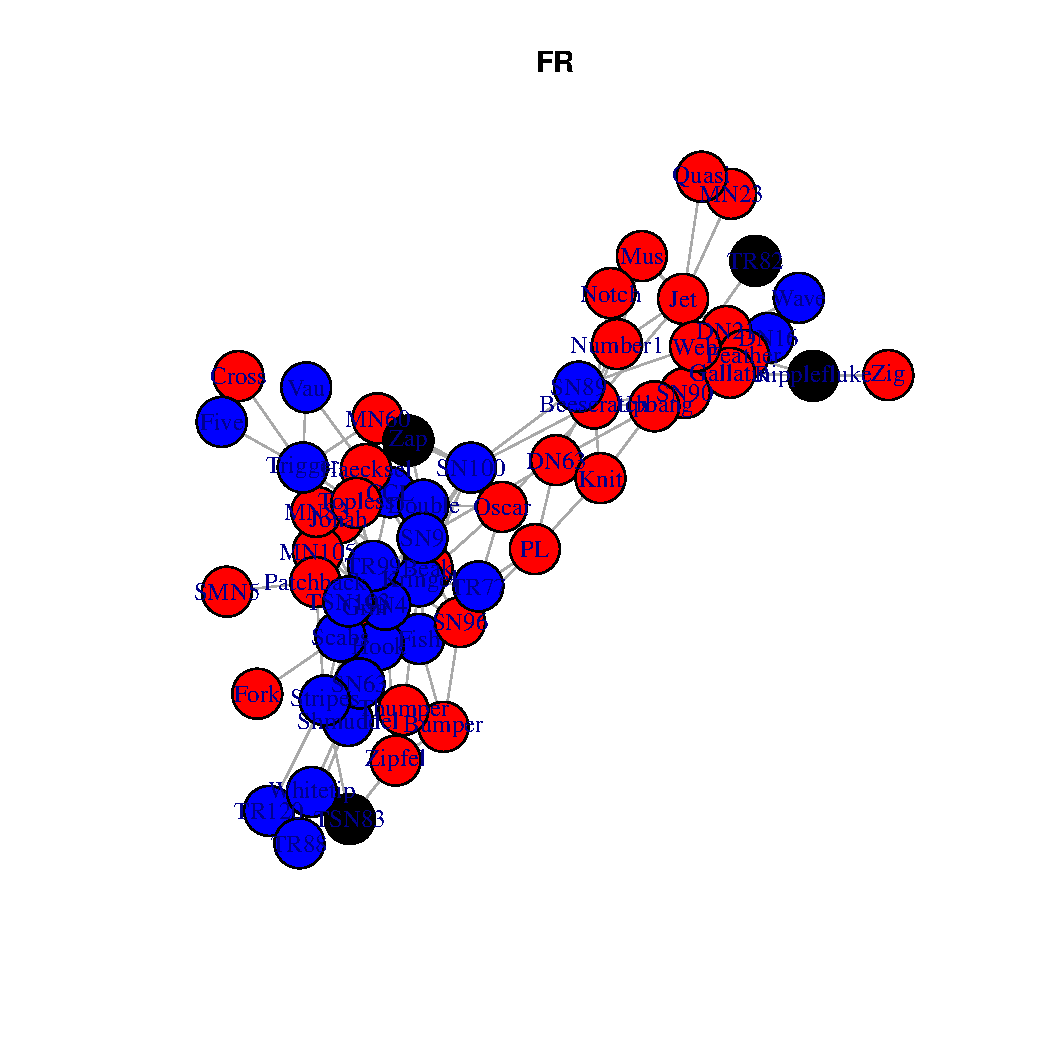
\includegraphics[width=1.0\linewidth]{Imagenes_P1/layout_dolphins2.pdf}
	\caption{Red de los delfines, graficada según \texttt{layout\_with\_fr}.}
	\label{pt2layoutsfr}
   \end{minipage}\hfill
   \begin{minipage}{0.3\textwidth}
	\centering
	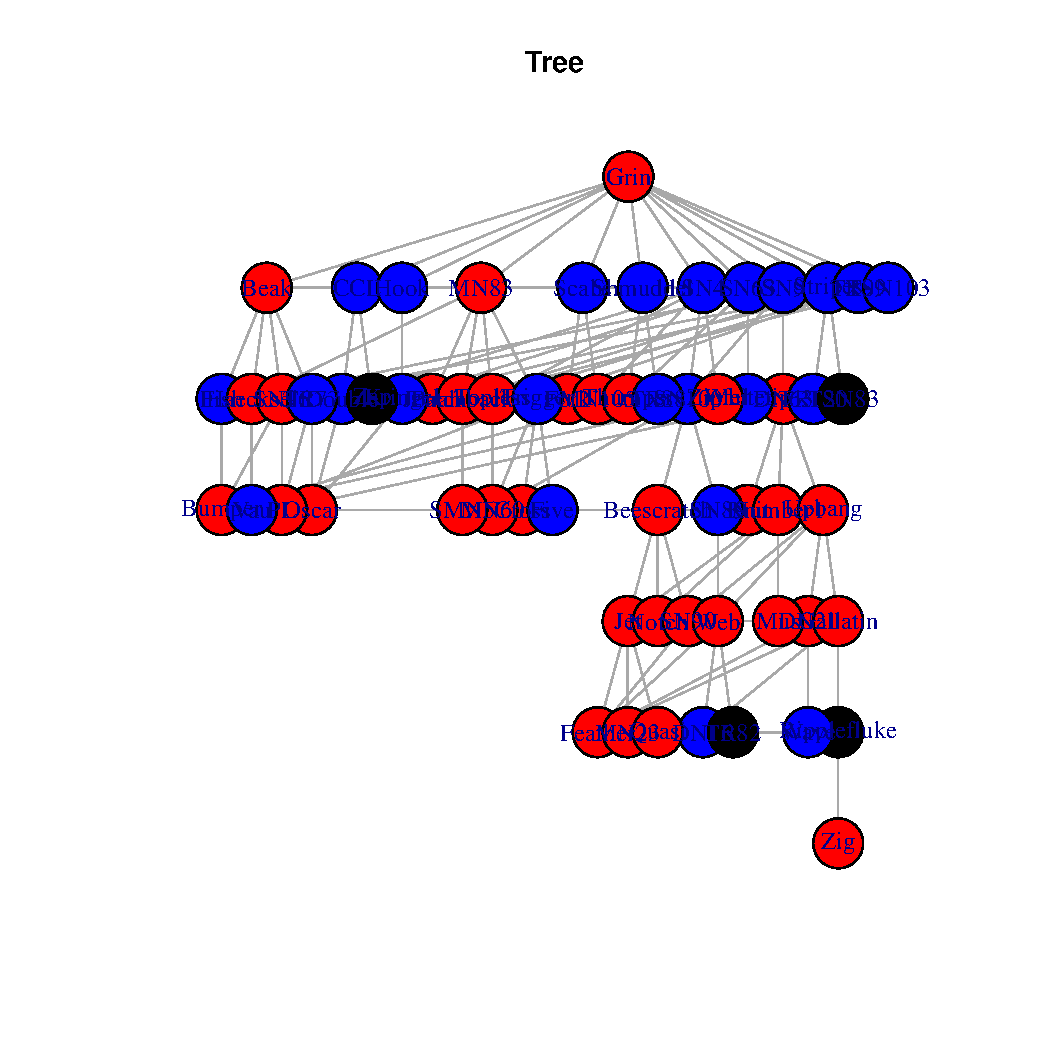
\includegraphics[width=1.0\linewidth]{Imagenes_P1/layout_dolphins3.pdf}
	\caption{Red de los delfines, graficada seg\'un \texttt{layout\_as\_tree}.}
	\label{pt2layouttree}
   \end{minipage}\hfill
   \begin{minipage}{0.3\textwidth}
	\centering
	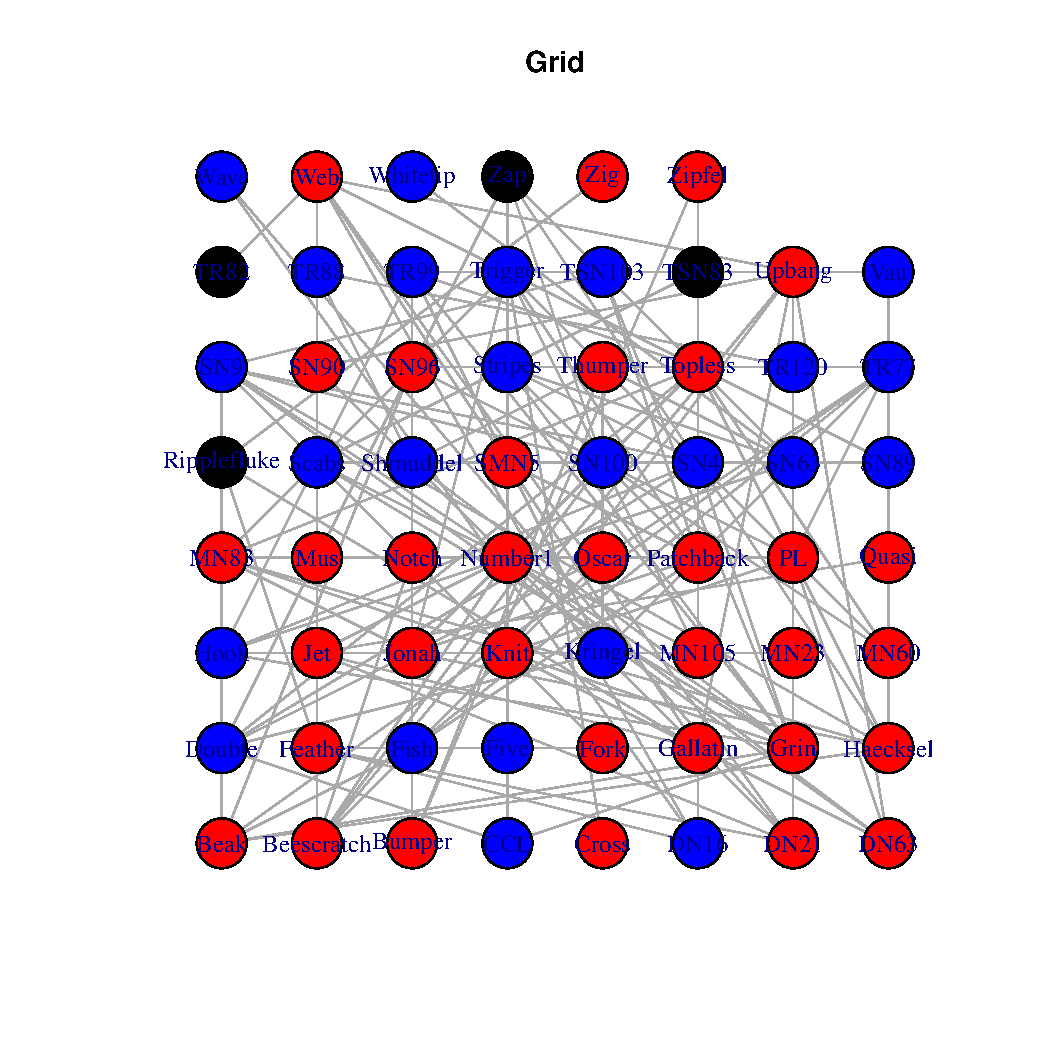
\includegraphics[width=1.0\linewidth]{Imagenes_P1/layout_dolphins7.pdf}
    \caption{Red de los delfines, graficada seg\'un \texttt{layout\_on\_grid}.}
	\label{pt2layoutgrid}
   \end{minipage}
\end{figure}


\subsection{Punto 2.b.}
En este punto se propone testear la hipótesis que sugiere \texttt{layout\_with\_fr}: que hay más vinculos entre delfines del mismo sexo (vinculos homofilos) que entre delfines de distinto sexo (vinculos heter\'ofilos). Para esto, calculamos la fracción de ejes que conectan delfines de distinto sexo como

\begin{equation}
    f_{mf} = \frac{1}{M}\sum_{ij} A_{ij} \delta_{s_i,m} \delta_{s_j,f}
\end{equation}

donde $s_i$ es el sexo del delfin $i$ y $A_{ij}$ es la matriz de adyacencia del red, y $M = \sum_{ij} A_{ij}/2$ es la cantidad de ejes en la red. De forma análoga, calculamos las fracciones de ejes que conectan hembras con hembras y machos con machos:

\begin{equation}
        f_{m} = \frac{1}{2M}\sum_{ij} A_{ij} \delta_{s_i,m} \delta_{s_j,m} 
\end{equation}
\begin{equation}
        f_{f} = \frac{1}{2M}\sum_{ij} A_{ij} \delta_{s_i,f} \delta_{s_j,f} 
\end{equation}
En todos los casos, consideramos únicamente los defines con sexo conocido. Obtenemos los valores de $f_{mf} = 0.327$, $f_{m} = 0.377$ y $f_{f} = 0.226$, quedando aproximadamente un $7\%$ de los ejes sin considerar por no conocerse el sexo. Para saber si estos valores son altos o bajos, el ejercicio propone reasignar de forma azarosa los sexos de cada delfín, y calcular las tres fracciones para cada asignación de sexo. Realizando 1000 reasignaciones, obtenemos tres distribuciones de valores. Podemos observar estos en las figuras \ref{pt2histo-cruces}, \ref{pt2histo-mym}, y \ref{pt2histo-fyf}. Obtenemos valores esperados de $\widehat{f_{mf}} = 0.43 \pm 0.04$, $\widehat{f_{m}} = 0.30 \pm 0.04$ y $\widehat{f_{f}} = 0.15 \pm 0.03$, de donde vemos que los valores observados se encuentran entre 1.8 y 2.8 sigmas de distancia de los esperados. Si calculamos los $p$ valores en cada caso, obtenemos $p_{mf} = 0.005$,$p_m = 0.029$ y $p_f = 0.015$, indicando una muy baja probabilidad de que por azar la estructura observada se forme.

\begin{figure}[!htb]
   \begin{minipage}{0.3\textwidth}
	\centering
	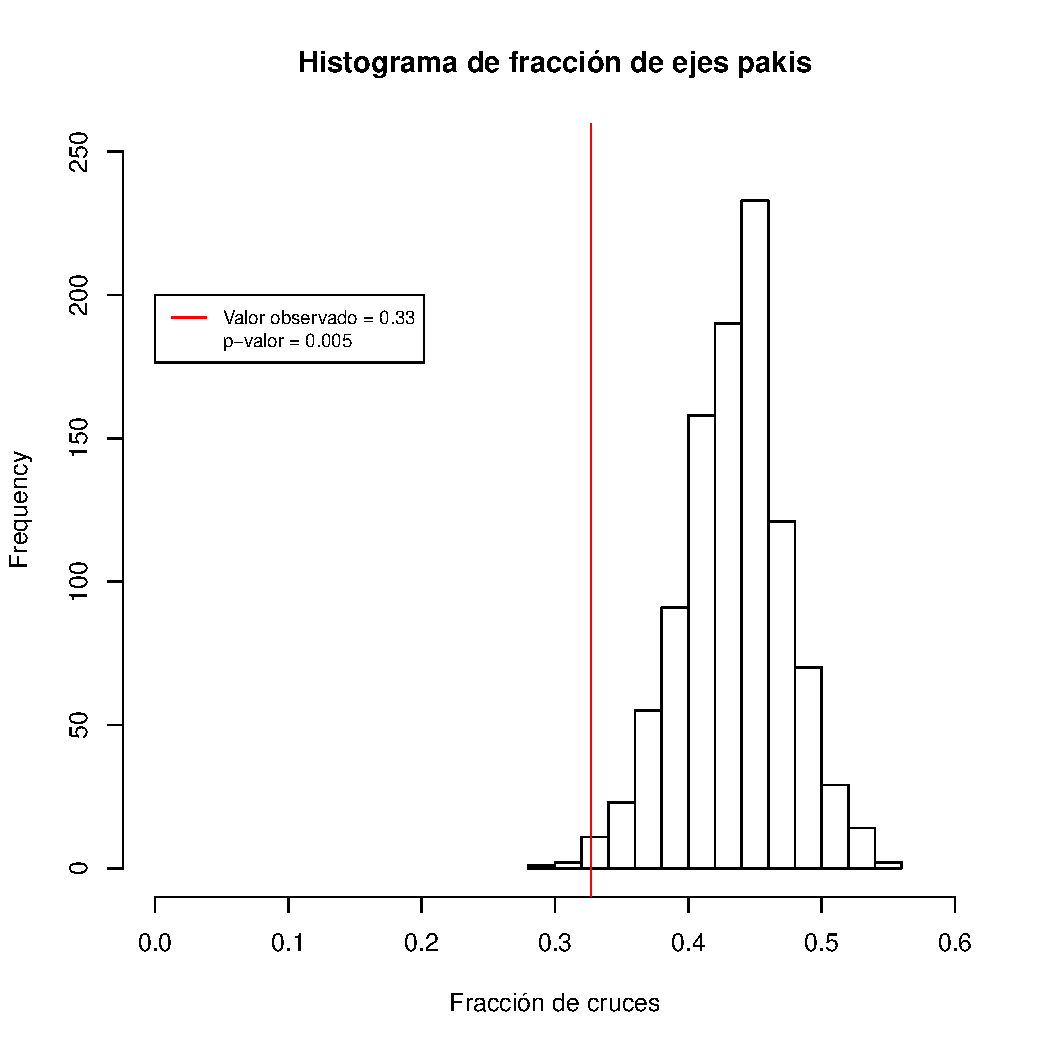
\includegraphics[width=1.0\linewidth]{Imagenes_P1/histo_homofilia1.pdf}
	\caption{Histograma de fracción de ejes que conectan delfines de sexos distintos.}
	\label{pt2histo-cruces}
   \end{minipage}\hfill
   \begin{minipage}{0.3\textwidth}
	\centering
	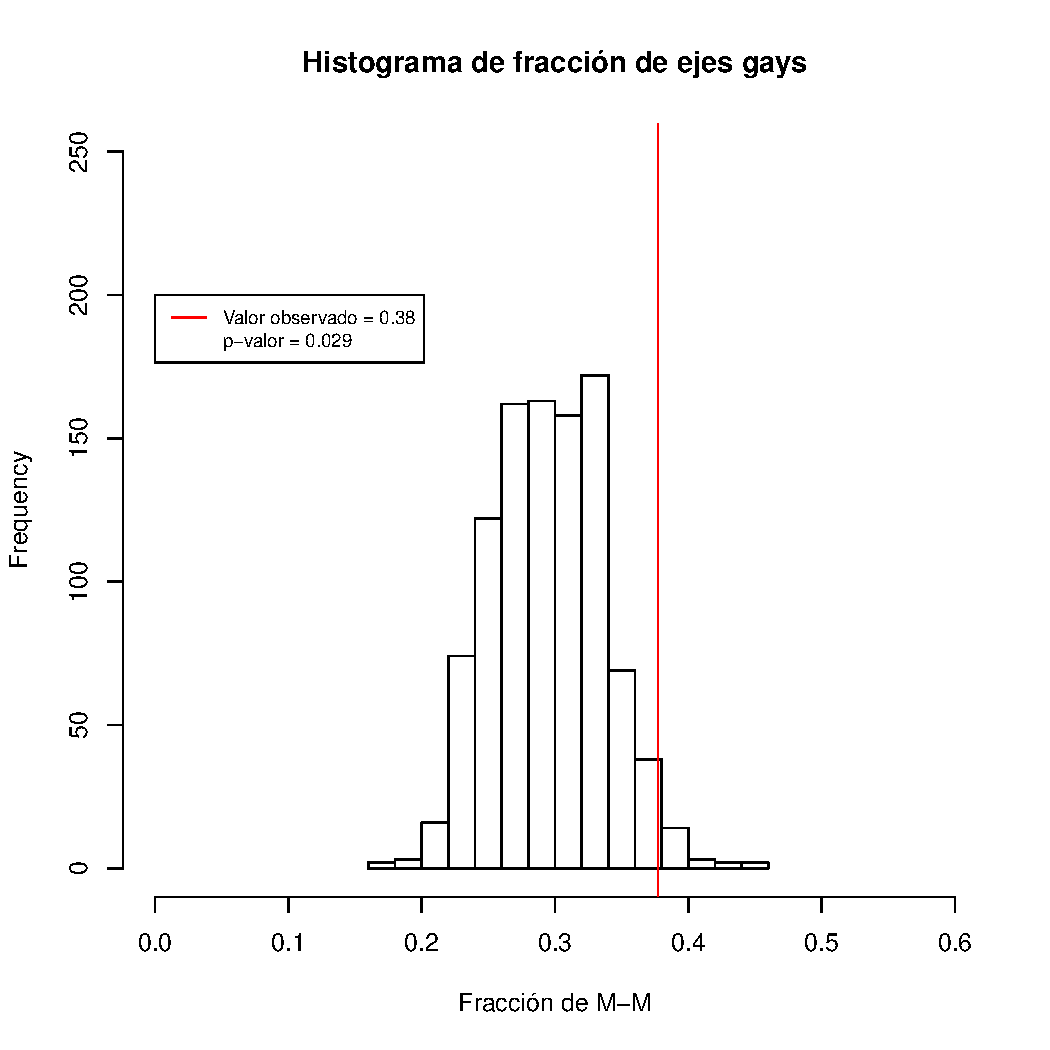
\includegraphics[width=1.0\linewidth]{Imagenes_P1/histo_homofilia2.pdf}
	\caption{Histograma de fracción de ejes que conectan defines macho con macho.}
	\label{pt2histo-mym}
   \end{minipage}\hfill
   \begin{minipage}{0.3\textwidth}
	\centering
	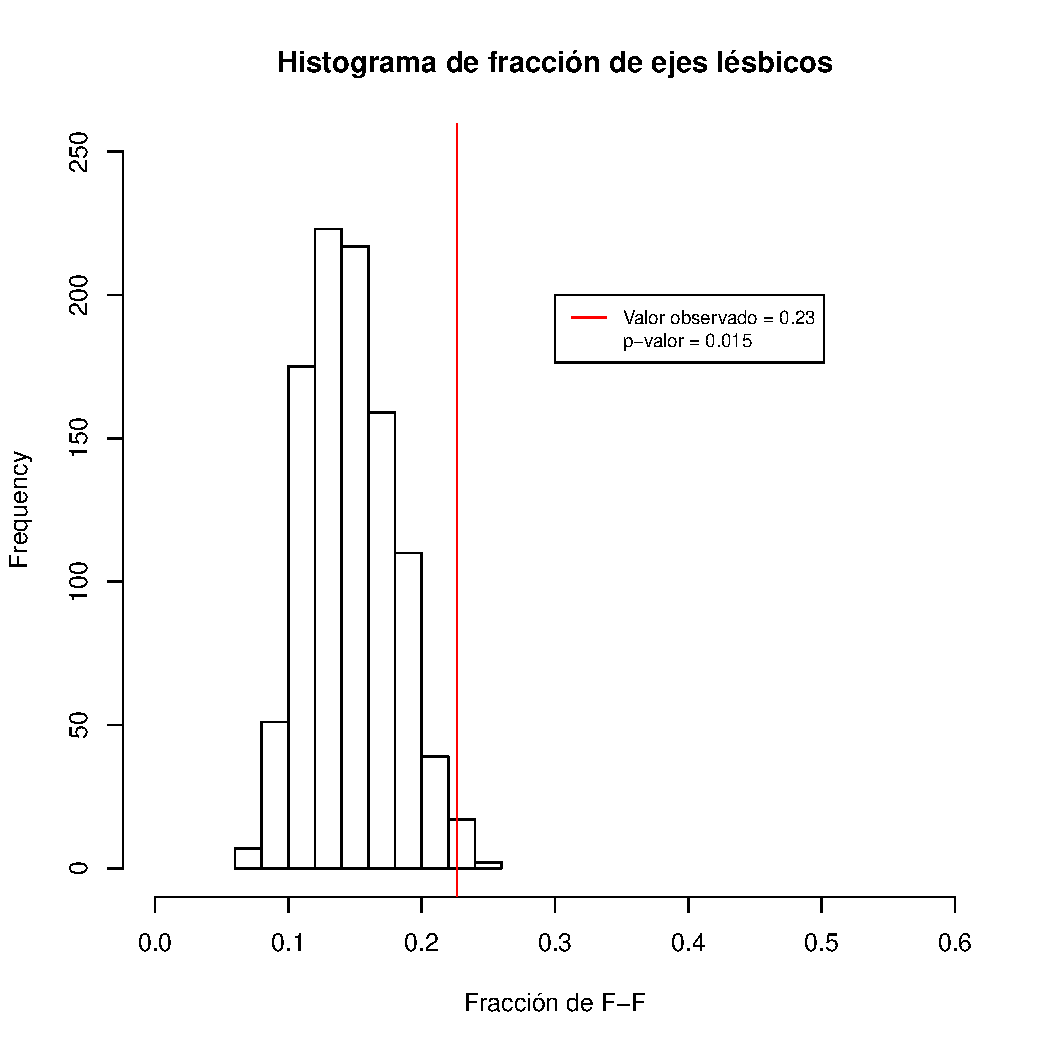
\includegraphics[width=1.0\linewidth]{Imagenes_P1/histo_homofilia3.pdf}
	\caption{Histograma de fracción de ejes que conectan defines hembra con hembra.}
	\label{pt2histo-fyf}
   \end{minipage}
\end{figure}

\subsection{Punto 2.c.}
Por último, el ejercicio propone comparar distintas estrategias para remover nodos de la red, basandose en la estructura de la misma. Para esto proponemos cuatro estrategias: extraer nodos según su grado, por su coeficiente local de clustering, por su betwenness (una medida de la cantidad de caminos mínimos que atraviezan un eje), o al azar. En la figura \ref{rupturas} podemos observar el tamaño de la primer y segunda componente. Elegimos la estrategia más apropiada viendo cual asemeja los tamaños más prontamente. Vemos que la estrategia más exitosa es la que extrae por betweenness. Seguida de ella está extraer por grado, que tiene éxito cuando las componentes ya son más pequeñas.

Por último, extraer según el coeficiente de clustering rinde resultados de tamaño mucho menor, habiendo desperdiciado la mayoría de las eliminaciones en formar componentes pequeñas en vez de partir la componente gigante en dos similares. No es sorprendente que este resultado sea muy parecido al azar.

\begin{figure}[!htb]
   \centering
   \begin{minipage}{0.6\textwidth}
    \centering
    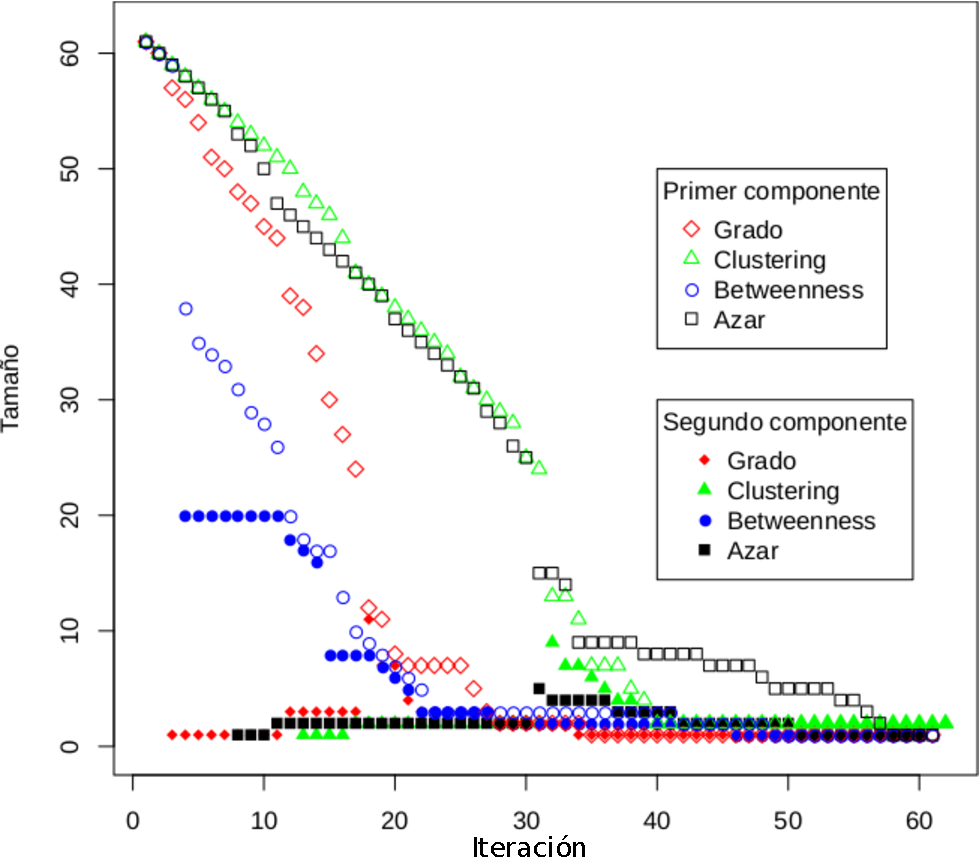
\includegraphics[width=1.0\linewidth]{Imagenes_P1/rupturas4.pdf}
    \caption{Decaimiento en el tamaño de la componente gigante y la segunda más grande a medida que se aplican algoritmos de destrucción basados en la eliminación de nodos por el grado de un nodo, por su coeficiente de clustering local, y por su betweenness. Cuando los puntos huecos de un color equivalen a los puntos llenos, se considera que se tienen dos componentes de igual tamaño como gigantes.}
    \label{rupturas}
   \end{minipage}
\end{figure}

\section{Problema 3}
En este ejercicio estudiamos la distribución de grados $P_k$ como función de $k$. Nuevamente utilizamos las funciones del paquete \texttt{igraph} de \texttt{R}, consiguiendo primero los grados de cada nodo y luego utilizando el comando \texttt{hist} 	que computa un histograma a partir del vector de grados.

En la siguiente tabla están los gráficos con distintas alternativas, con bineado lineal o logarítmico y utilizando diferentes escalas.

\begin{figure}[!htb]
   \begin{minipage}{0.3\textwidth}
	\centering
	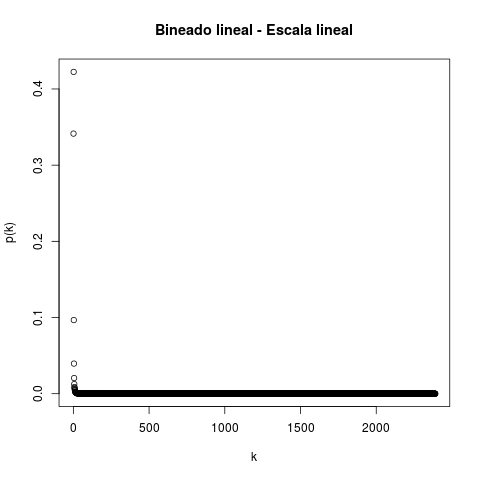
\includegraphics[width=1.0\linewidth]{Imagenes_P3/P3_binlin_lin.png}
	\caption{Bineado Lineal - Escala lineal}
	\label{pt3linlinlin}
   \end{minipage}\hfill
   \begin{minipage}{0.3\textwidth}
	\centering
	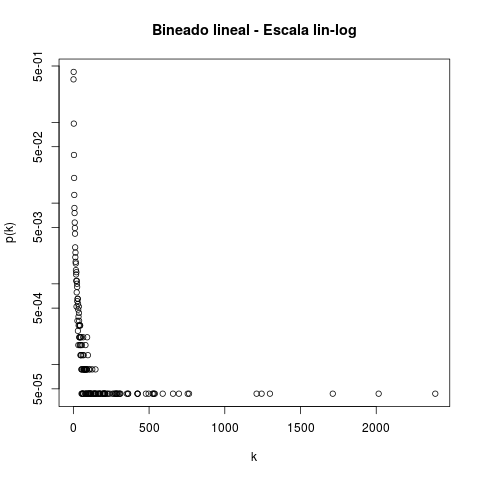
\includegraphics[width=1.0\linewidth]{Imagenes_P3/P3_binlin_linlog.png}
	\caption{Bineado Lineal - Escala lineal en x logarítmica en y}
	\label{pt3linlinlog}
   \end{minipage}\hfill
   \begin{minipage}{0.3\textwidth}
	\centering
	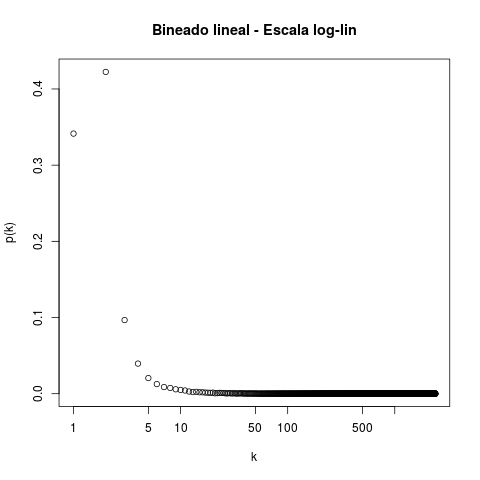
\includegraphics[width=1.0\linewidth]{Imagenes_P3/P3_binlin_loglin.png}
	\caption{Bineado Lineal - Escala logarítmica en x lineal en y}
	\label{pt3linloglin}
   \end{minipage}\hfill
      \begin{minipage}{0.3\textwidth}
	\centering
	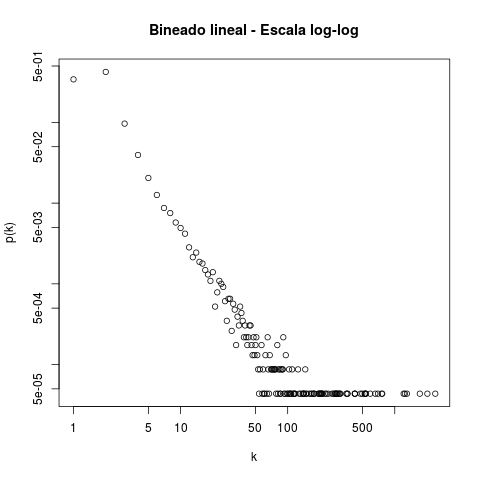
\includegraphics[width=1.0\linewidth]{Imagenes_P3/P3_binlin_loglog.png}
	\caption{Bineado Lineal - Escala logarítmica}
	\label{pt3linloglog}
   \end{minipage}\hfill
      \begin{minipage}{0.3\textwidth}
	\centering
	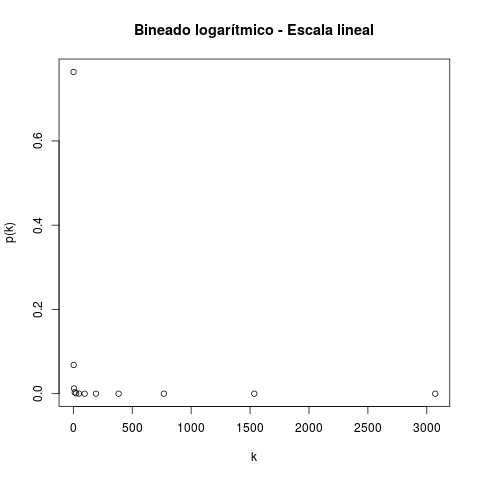
\includegraphics[width=1.0\linewidth]{Imagenes_P3/P3_binlog_lin.png}
	\caption{Bineado logarítmico - Escala lineal}
	\label{pt3loglin}
   \end{minipage}\hfill
      \begin{minipage}{0.3\textwidth}
	\centering
	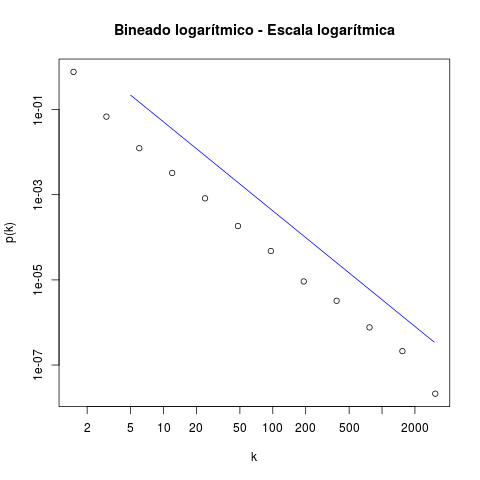
\includegraphics[width=1.0\linewidth]{Imagenes_P3/P3_binlog_log.png}
	\caption{Bineado logarítmico - Escala logarítmica - Con recta del ajuste PL}	
	\label{pt3loglog}
   \end{minipage}\hfill
   \label{pt2layout}
\end{figure}

En las figuras 4 a 6 podemos ver la distribución de grados utilizando un bineado lineal. Se se aprecia la forma de la distribución aunque es complicado cuantificar si un ajuste libre de escala será coherente. En figuras \ref{pt3loglin} y \ref{pt3loglog} se utilizó un bineado logarítmico en base 2, y en la escala logarítmica se aprecia bien el carácter libre de escala de dicha distribución.

En la figura \ref{pt3loglog} se agregó la recta de ajuste libre de escala obtenida vía el comando \textit{fit\_power\_law} utilizando una malla de $3000$ puntos a partir del $k_{min}$ que en nuestro caso toma valor $5$. El valor estimado es $\alpha=2.097157$ ajustandose correctamente aunque corrido hacia arriba. Esto se debe a que el parámetro de normalización, es decir, la ordenada al origen, se calcula teniendo en cuenta todos los valores de grado, no solo los mayores al $k_{min}$.

\section{Problema 4}
En el cuarto problema se propone realizar distintas medidas para analizar la asortatividad de una red. La asortatividad representa la tendencia de un nodo a parecerse topológicamente a sus vecinos (por ejemplo en términos de grado). Para esto se toman en consideración dos redes: \textit{netscience} y \textit{as\_july\_22}. La primera es una red de colaboraciones científicas y la segunda de internet.

\subsection{Punto 4.a.}
El primer cálculo que se propone para observar la asortatividad es calcular el valor de $k_{nn}(k)$, que es el valor medio del grado de los vecinos de los nodos de grado $k$. En las figuras \ref{pt4july} y \ref{pt4netscience} podemos observar los valores de $k_{nn}(k)$ en función de $k$. Siguiendo la propuesta de Newmann, podemos hacer un ajuste lineal de $\log(k_{nn}(k) \sim \log (k)$, para obtener el coeficiente $\mu$, donde

\begin{equation}
k_{nn}(k) = A k^\mu
\end{equation}
Siguiendo este modelo, obtenemos los valores 

\begin{equation}
\mu_{july} = -0.44 \pm 0.04
\end{equation}
\begin{equation}
\mu_{netsci} = 0.31 \pm 0.07 
\end{equation}
de donde podemos ver que la red \textit{as\_july\_22} es desasortativa (es decir, que nodos con grados altos tienden a juntarse con nodos con grado bajo), y la red \textit{netscience} es asortativa, juntandose nodos con grados altos con otros con grados altos. Este resultado pareciera tener sentido bajo la siguiente visión: en la red \textit{as\_july\_22} tenemos nodos con grado muy alto, que son centrales a la conectividad de la red de internet. Todos los nodos de grado bajo se conectan a ellos ya que funcionan como una central de comunicación. En cambio, en la red \textit{netscience}, que es de coautoria de papers, un nodo con grado alto representa un científico muy productivo. En esta red es esperable que dos científicos trabajen juntos mientras más productivos sean, por lo cual tiene una asortatividad alta.

A continuación, se propone medir la asortatividad con otro coeficiente, propuesto por Newman, según la ecuación:

\begin{equation}
r = \frac{\sum_{ij}(A_{ij}-k_i k_j/2m)k_i k_j}{\sum_{ij}(k_i\delta_{ij} -k_i k_j /2m)k_i k_j}
\end{equation}
Este coeficiente permite medir la tendencia lineal, pero en escala natural (no logaritmica). Para ambas redes, obtenemos en este caso:
\begin{equation}
r_{july} = -0.19
\end{equation}
\begin{equation}
r_{netsci} = 0.46 
\end{equation}
de forma tal que ambos coeficientes apuntan a las mismas conclusiones.


\begin{figure}[!htb]
\centering
   \begin{minipage}{0.4\textwidth}
	\centering
	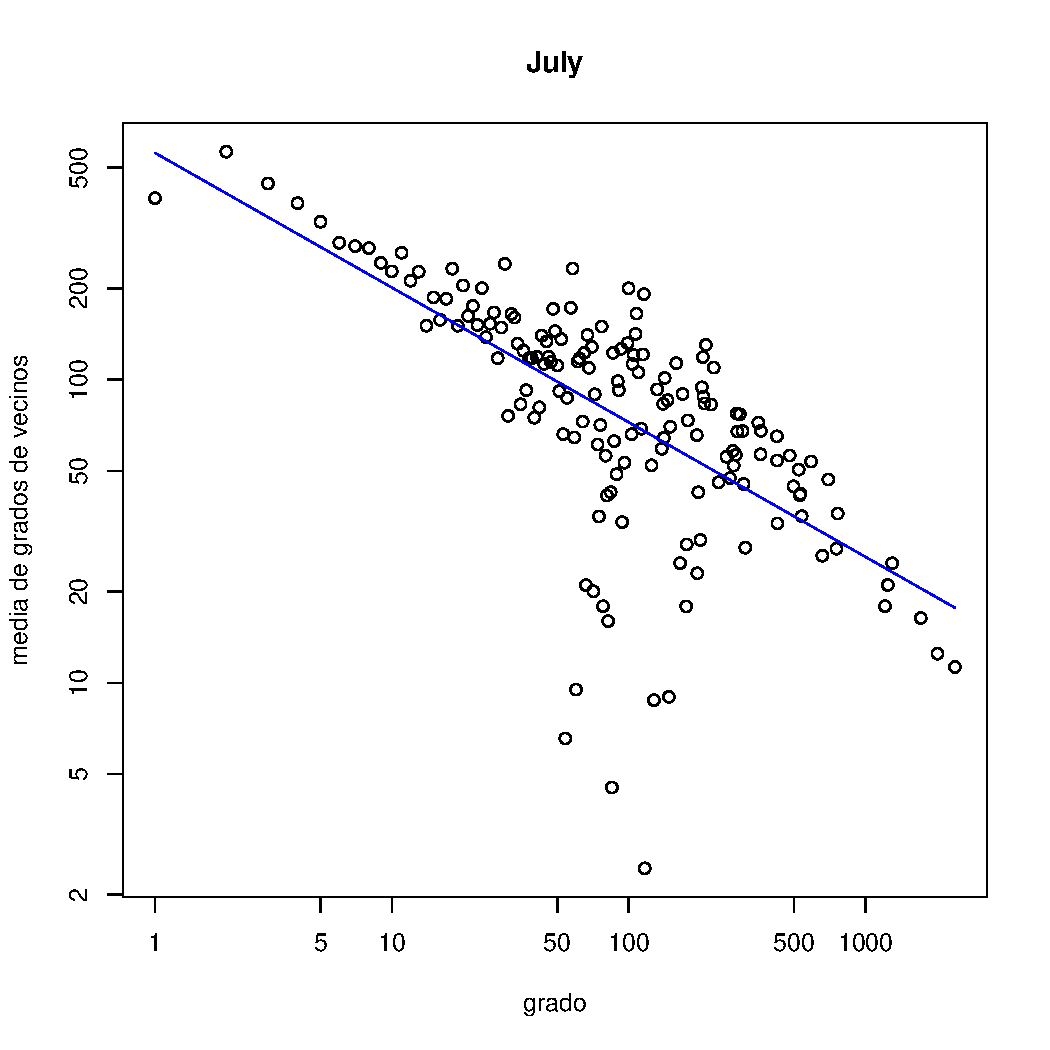
\includegraphics[width=1.0\linewidth]{Imagenes_P4/ej42}
	\caption{Valores de $k_{nn}(k)$ en función del grado $k$ para la red \textit{as\_july\_22}. En azul la regresión lineal.}
	\label{pt4july}
   \end{minipage}
   \hspace{50px}
   \begin{minipage}{0.4\textwidth}
	\centering
	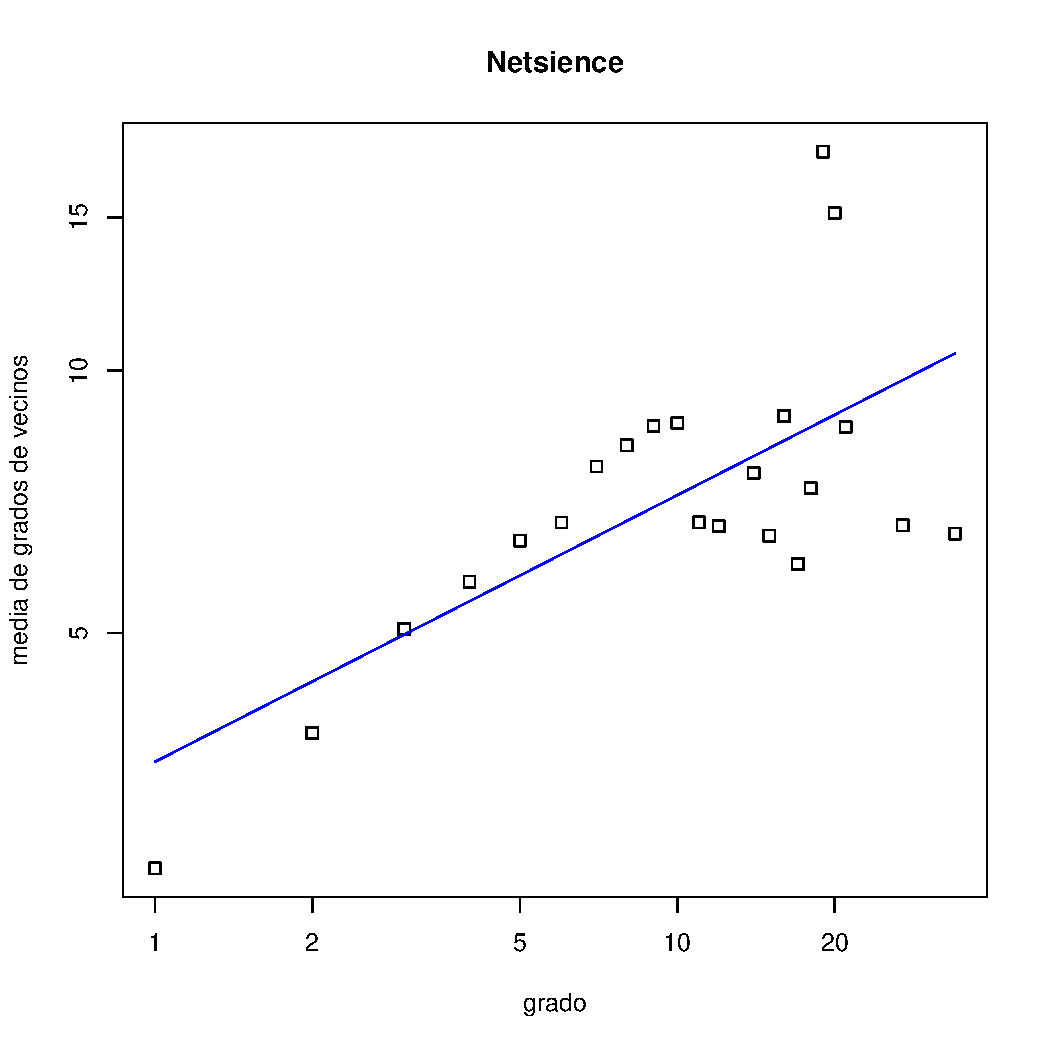
\includegraphics[width=1.0\linewidth]{Imagenes_P4/ej44}
	\caption{Valores de $k_{nn}(k)$ en función del grado $k$ para la red \textit{netscience}. En azul la regresión lineal.}
	\label{pt4netscience}
   \end{minipage}
\end{figure}

\subsection{Punto 4.b.}
Por último, se propone repetir las medidas para las redes de interacción de proteinas de levadura Y2H y AP-MS presentadas en el punto 1. En las figuras \ref{pt4y2h} y \ref{pt4apms} se encuentran graficados los valores de $k_nn(k)$ en función de $k$ con sus regresiones lineales en escala log-log.

En este caso los datos están más dispersos, por lo que la calidad de las regresiones disminuye. Obtenemos los valores:
\begin{equation}
\mu_{Y2H} = -0.26 \pm 0.15
\end{equation}
\begin{equation}
\mu_{APMS} = 0.39 \pm 0.12 
\end{equation}
\begin{equation}
r_{Y2H} = -0.04
\end{equation}
\begin{equation}
r_{APMS} = 0.60 
\end{equation}
donde nuevamente vemos acuerdo entre los coeficientes $r$ y $\mu$, aunque en el caso de la red Y2H la correlación es muy baja. En este caso,vemos que la red Y2H es desasortativa, y la red APMS es asortativa. Dado que la red Y2H se construye a partir de interacciones binarias, únicamente aquellas proteinas que interactuan con muchas otras tendrán muchas conexiones. En cambio, en la red APMS se establecen conexiones entre los grupos de conexiones que pertenecen a un complejo proteico común. Esto facilita la vinculación entre nodos de grado alto en la red APMS, ya que proteinas que interactuan con muchas otras (menos interactuantes), terminaran conectadas igualmente, al encontrarse con alta probabilidad ambas en un complejo proteico grande (ya que ambas son muy interactuantes). Cabe notar que en el caso de APMS es muy marcado como a grados altos hay mucha dispersión en el grado medio de los vecinos, indicando que no todas las \textit{proteinas famosas} se conectan principalmente con otras \textit{proteinas famosas}

\begin{figure}[!htb]
\centering
   \begin{minipage}{0.4\textwidth}
	\centering
	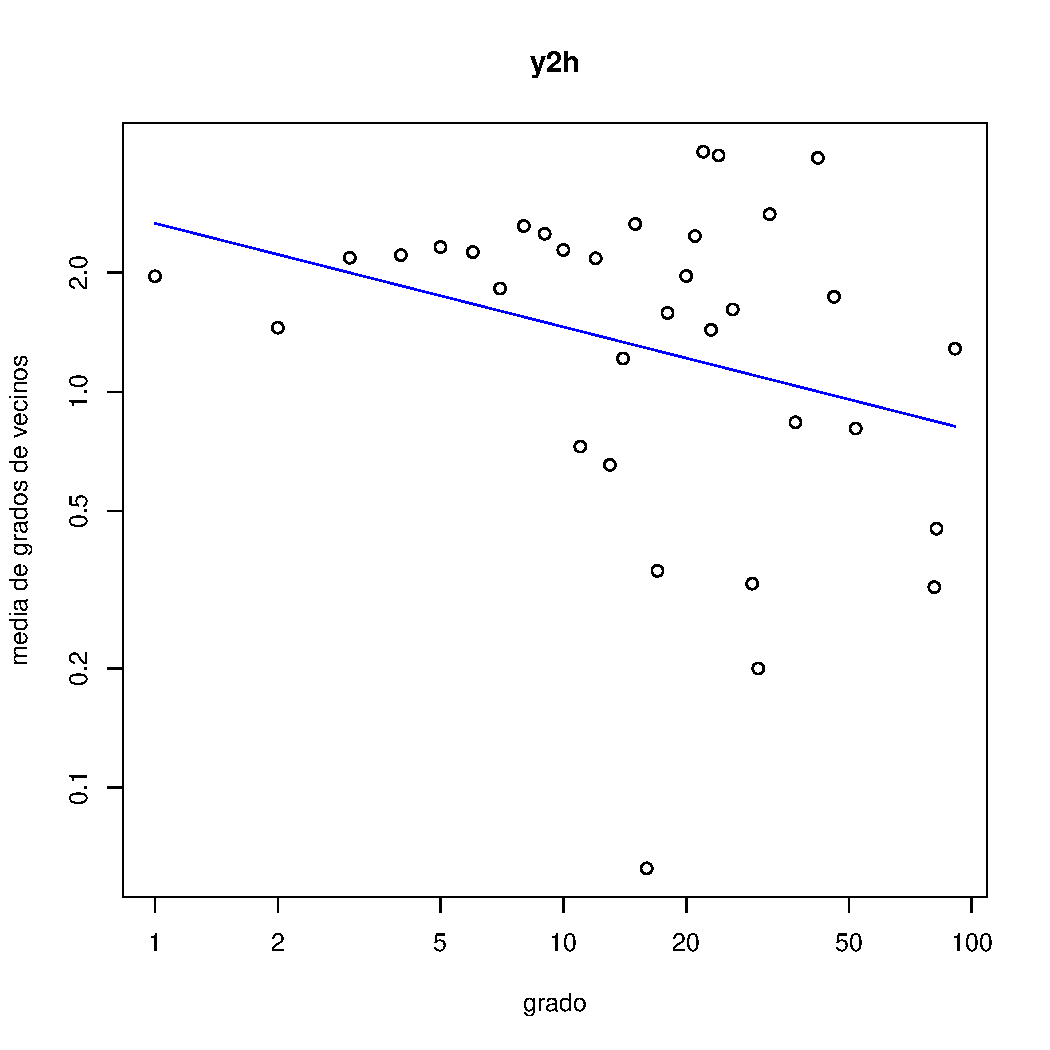
\includegraphics[width=1.0\linewidth]{Imagenes_P4/ej46}
	\caption{Valores de $k_{nn}(k)$ en función del grado $k$ para la red \textit{Y2H}. En azul la regresión lineal.}
	\label{pt4y2h}
   \end{minipage}
   \hspace{50px}
   \begin{minipage}{0.4\textwidth}
	\centering
	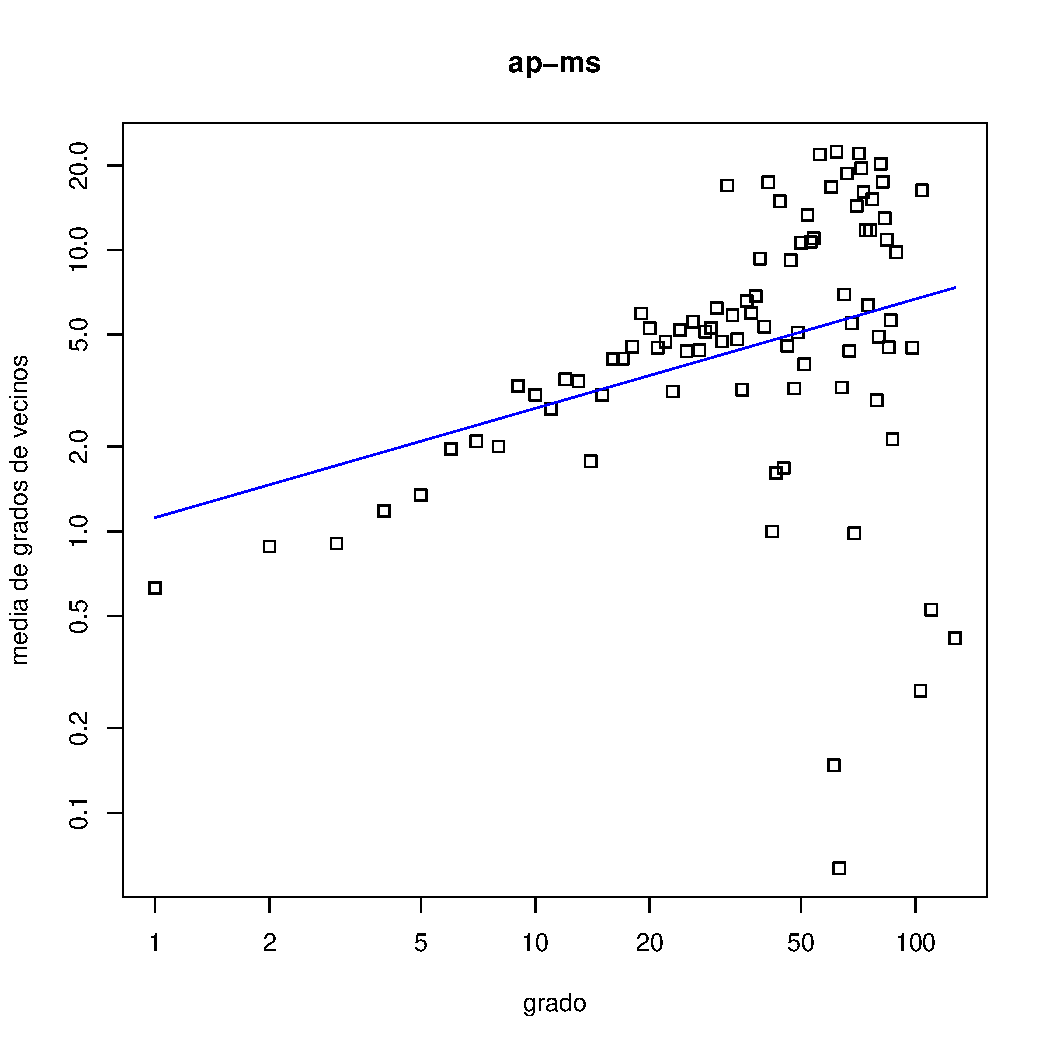
\includegraphics[width=1.0\linewidth]{Imagenes_P4/ej48}
	\caption{Valores de $k_{nn}(k)$ en función del grado $k$ para la red \textit{AP-MS}. En azul la regresión lineal.}
	\label{pt4apms}
   \end{minipage}
\end{figure}

\end{document}
